\chapter{Experimental Setup and execution}
\section{Setup}
The experiment consists of a probe made from Gallium-Arsenide that is produced in such a way to produce an atomically flat surface between the GaAs
and the insulator, so that an electron gas can form that has only few disturbances.

The probe has 6 electrical contacts of which most of them did not work for this run. For this reason the contacts 5, 2 and 1 where used. The contacts
5 and 2 where used to measure $U_{xy}$ and the contacts 5 and 1 where used to measure $U_{xx}$. The geometry of the probe can be seen in
\ref{fig:probe}.
\begin{figure}[tb]
	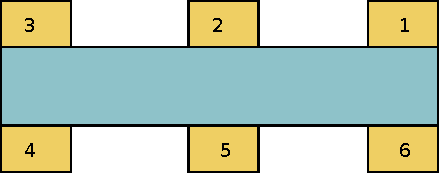
\includegraphics[width=\textwidth]{fig/QEH-probe.pdf}
	\caption{The geometry of the probe. The yellow areas are the contact points}
	\label{fig:probe}
\end{figure}

To be able to observe the QEH, the probe must be cooled as low as possible to reduce the effect of thermal noise on the measurements. Furthermore the
QHE is dependent on a magnetic field. The stronger the magnetic field can be made, the more pronounced the effect is. Because of this, a
superconducting Niob-Titanium magnet is used to produce a field of 6 Tesla at the probe. As NbTi magnets only become superconducting below the
temperatures of liquid nitrogen, liquid helium is used to cool the probe and the magnet. This lowers the probe temperature to 4K under atmospheric
pressure and can be lowered to 2K when the probe chamber is evacuated. For this a vacuum pump is connected to the probe chamber and used for parts of
the experiment.

The assembly of magnet, probe, probe chamber, dewar and connectors is depicted in \ref{fig:setup}.
\begin{figure}[h]
    \centering
    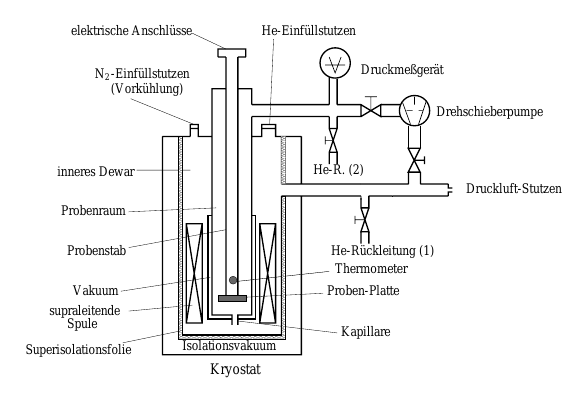
\includegraphics[width=15.8cm]{fig/setup.png}
	\caption{The experimental setup. The probe and Magnet are inside the isolating dewar. The probe chamber is isolated against the Superconducting
	magnet and connected to the bath of liquid helium through a capillary.}
	\label{fig:setup}
\end{figure}

The probe chamber and the surrounding vessel containing the magnet and the bath of liquid helium are connected to a vacuum pump. The gaseous helium is
also collected through the return valve of the setup to a helium recovery system.

\section{Execution}
To begin the experiment, the chamber and the dewar need to be brought down to a Temperature of 4K.
As both nitrogen and oxygen become solid at those temperatures and could clog the capillary, both chambers need to be flushed with helium. To do this
both vessels are evacuated and then the helium return valve is opened, letting helium fill the evacuated space. This procedure is repeated twice.

Unfortunately, during the filling of the liquid nitrogen, the chamber was still evacuated and the removal of a plug let air enter the evacuated and
flushed chamber. Due to this the process needed to be repeated.

After slowly filling the dewar with Nitrogen, the nitrogen was left sitting in the dewar to let the dewar cool to the 77K boiling point of Nitrogen.
To be able to refill the dewar with Helium the nitrogen is first blown out, using it's evaporation pressure. To fill the Helium, a vacuum insulated
metal tube is used to minimize the evaporation of helium.

After the helium was filled, we waited another 30 minutes for the dewar to cool to the 4K Boiling point of Helium and began to observe the resistance
of the carbon resistor that acted as a thermometer.

Either due to lack of patience or some kind of blockage of the capillary the temperature did not reach below 20$\circ$ K as indicated by the resistor.
To reduce the temperature, the vacuum pump was started and connected such that it evacuated the helium reservoir lowering it's boiling point and
hopefully cooling the probe to the desired temperature. This procedure was repeated multiple times, getting the temperature down to 4.1$\circ$K at the
lowest point.

At that point it was decided to start a measurement, even though the temperature drift was significant ($>1\circ$).

